

\documentclass[runningheads,a4paper]{llncs}

\usepackage{amssymb}
\setcounter{tocdepth}{3}
\usepackage{graphicx}
\usepackage{amsmath}
%\usepackage{amsfonts}
%\usepackage{amsthm}
\usepackage{subfigure}
%\usepackage{caption}
%\usepackage{subcaption}
%\usepackage{cite}
\usepackage{hyperref}
\usepackage{url}
\urlstyle{same}
\newcommand{\keywords}[1]{\par\addvspace\baselineskip
\noindent\keywordname\enspace\ignorespaces#1}

\makeatletter
\let\c@lemma=\c@theorem
\let\c@corollary=\c@theorem
\let\c@fact=\c@theorem
\makeatother

\let\realendproof=\endproof
\def\endproof{\hspace*{\fill}$\Box$\realendproof}


\begin{document}

\mainmatter  

\title{Ghost gets Harder when Played in German}
\titlerunning{Ghost gets Harder when Played in German}

\author{Fermi Ma
\and Matt Susskind \and Erik Waingarten}
%
\authorrunning{Fermi Ma \and Matt Susskind \and Erik Waingarten}
% (feature abused for this document to repeat the title also on left hand pages)

% the affiliations are given next; don't give your e-mail address
% unless you accept that it will be published
\institute{MIT Computer Science and Artificial Intelligence Laboratory,\\
32 Vassar St., Cambridge, MA 02139, USA, \\
\protect\url{{fermima,msuss,eaw}@mit.edu}}

%
% NB: a more complex sample for affiliations and the mapping to the
% corresponding authors can be found in the file "llncs.dem"
% (search for the string "\mainmatter" where a contribution starts).
% "llncs.dem" accompanies the document class "llncs.cls".
%

\maketitle


\begin{abstract}

Ghost is a popular word game played by two or more players. Players take turns adding a letter to the end of a word fragment, trying not to be the first to complete a valid word. We show that the game, when played on a regular language, is PSPACE-complete, and extend the result to three variants of the game. In addition, we take advantage of a quirk of the German language --- that German words can be concatenated together to form longer words --- to give a fun extension of our proof of PSPACE-hardness to subsets of the German language. 
\end{abstract}

\keywords{algorithmic combinatorial game theory, mathematical games and puzzles, computational complexity}

\section{Introduction}

	Ghost is a game typically played on a human language such as English. A player starts the game by picking a letter of the alphabet, and play continues as the players take turns adding letters to the end of the current string. At every point in time, the string of letters must be the prefix of some valid word, and if this is not the case, another player can make a challenge. Usually, the game is played with a score, where each loss gives a player a letter of the word ``Ghost", and thus the first person to lose five games loses the game.

	In this paper, we analyze a simple version of the game where we assume each player has perfect knowledge of the dictionary, and no score is kept (only one round is played). If the entire dictionary of the game is given in unsimplified form, the game is considered to be solved; the game tree of all combinations can be searched for a winning strategy in polynomial time with a minimax algorithm \cite{ghostbusters}\cite{randall}. Thus, we consider a version of the game played on regular languages, as this allows a large input dictionary for the game to be given as a much smaller regular expression.

%
%Alan Frank and Randall Munroe have ``solved" the game by finding a winning strategy for the first player in the Official Scrabble Players Dictionary and on the Ubuntu dictionary \cite{ghostbusters} \cite{randall}. 


	Our first result is that playing the classic version of Ghost on a regular language is PSPACE-complete. We also extend this result to three variants of ghost, namely Superghost, Superduperghost, and XGhost. Our second result is that playing Ghost on any subset of the German language given by a regular expression is also PSPACE-complete. We focus on the German language because it allows words to be concatenated together, a feature that drastically impacts play of games such as Ghost.

%
%	Ghost is a word game in which two players take turns adding a letter to the end of a word fragment, trying to not be the first to complete the word. The game is usually played by a group of over 2 people, usually on a long roadtrip. According to Wikipedia, the game has received some media attention. It has been referenced in several American television shows like a 1962 episode of ``Car 54, Where Are You?", a 2003 episode of Buffy The Vampire Slayer, and Ghostwriter. It has also appeared in the January 10, 1974 Doonesbury comic strip, Chapter 7 of Richard Bachman's ``The Long Walk", and ``The Deer Park" by Norman Mailer.
%
%	Our first result is that given a regular language, it is PSPACE-complete to determine whether a given player has a winning strategy when playing with that language. We use the first result to prove an analogous result for a specific language. In particular, we show that when the game is played on subsets of the German language, it is PSPACE-complete to determine whether a given player has a winning strategy. The same results hold for common variations of the game.

\section{Game Definitions}
\label{Game Definitions}

\subsection{Rules for the Classic Game}

	The game allows for two or more players, but we restrict our attention to the two-player version. One player starts the game by playing a letter, and then the players alternate adding letters until a valid word is formed. At each turn the current word fragment must be the prefix of some valid word, and thus playing a letter that does not give a word prefix is considered an invalid move. A player wins the game when his/her opponent completes a valid word. 

% 
%	Thus, the game only becomes interesting from a computational standpoint when the number of words is large. This motivates the need to look at other ways of representing subsets of words. In this paper, we use regular expressions to represent sets of words that are much larger than the input size (the length of the regular expression). A regular expression can work like a dictionary which confirms whether words are in the language.

\subsection{Variants}

There are some popular variants of the regular rules:

\textbf{Superghost}: Same as regular Ghost, but letters can also be added to the front of the word fragment.

\textbf{Superduperghost}: Same as Superghost, but before playing a letter, a player can choose to reverse the word fragment.

\textbf{Xghost}: Players can add letters anywhere in the word fragment, including between letters.

\textbf{Spook}: Players add letters to a bag of words, trying to avoid any permutation of the letters to form a word. 

\subsection{Regular Expressions}

We assume the game is played on a dictionary defined by a regular expression. 

\section{Hardness of Classic Ghost}
\label{Hardness of Classic Ghost}

We consider the following instance of the game:

\vbox{
\noindent
\begin{quote}
Given any regular expression $R$ and players 1 and 2, does player 1 have a winning strategy in Ghost when played in the language generated by $R$? Player 1 starts.
\end{quote}
}

\begin{theorem}
Determining whether player 1 has a winning strategy when Ghost is player over regular languages is in PSPACE. 
\end{theorem}

\begin{proof}
Suppose that the regular expression has length $n$, and that we can build an NFA with $m$ states were $m$ is a polynomial of $n$. We first claim that a winning strategy will take at most $m$ turns. This is because if we follow a game by keeping the markers on the current states in the NFA, then a winning strategy never goes through a loop. 

If there is a winning strategy that goes through a loop, then if the loop length is even, there was no need to go through the loop. If the loop length is odd, then the game will continue going through the loop forever since a symmetric situation will arise once the loop is over.

Therefore, we can solve the game by a fully-quantified boolean formula where variables represent choices for the two players. We can check whether pairs of letters are said correctly and whether player 1 wins in a polynomially long formula \cite{theoryofcomp}. 
\end{proof}

\begin{theorem} Determining whether player 1 has a winning strategy when Ghost is played over regular languages is PSPACE-hard.
\end{theorem}
\begin{proof} We prove this via reduction from Generalized Geography, a problem known to be PSPACE-hard \cite{theoryofcomp}. Recall that the problem is set up as follows:
Players 1 and 2 take turns moving a token from vertex to vertex in a directed graph G, where player 1 starts the token at a specified start node $s$. A player loses when they are unable to move the token to a vertex that did not have a token previously. Given an instance of the problem, $(G,s)$, can player 1 win the game?

We will use the graph $G$ to build a non-deterministic finite automaton (NFA) that will give a regular expression to play Ghost with. This construction will give an equivalence between games played in Generalized Geography and Ghost, so a winning strategy in one will correspond to a winning strategy in the other and vice versa. To do so, we first label all the edges of $G$ arbitrarily. These labels will represent transitions in the NFA.

We start building the NFA by redrawing the graph $G$, except as a diagram for the NFA. This means that vertices of $G$ are drawn as states of the NFA, and the directed edges turn into transitions between states where transitions are labeled with the same labels given to the corresponding edges in $G$. We then extend construction: for each node $x\in G$, we make another copy of $G$, which we call $G_x$, and make it part of the NFA. For any directed edge $(x,a)$ pointing away from $x$ with label $l$, we make a transition from $x$ to $a'$ in $G_x$ with label $l$, where the prime denotes a corresponding vertex in $G_x$. In addition, we make $x' \in G_x$  the only accept state among the states in $G_x$. If $x\in G$ has no outgoing edges, then corresponding $x$ state in the NFA will have a transition to an accept state $y$ labeled with all possible labels. An example of the contruction is given in Figure~\ref{fig:instance} and Figure~\ref{fig:reduction}. In Figure~\ref{fig:reduction}, the solid transitions correspond to the transitions from $G$ and the dashed transitions correspond to the transitions to the copies of $G$.

From this NFA, we can generate an equivalent regular expression in polynomial time \cite{theoryofcomp}.
\begin{figure}[ht]
\centering
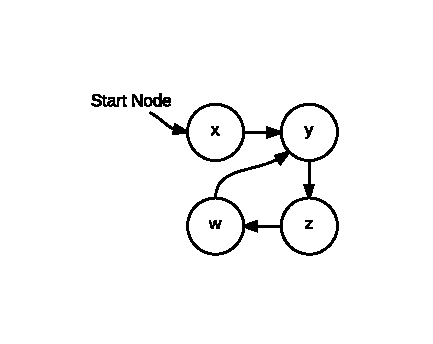
\includegraphics[width=0.3\linewidth]{Ghost1.pdf}
\caption{Instance of Generalized Geography}
\label{fig:instance}
\end{figure}

We claim that a winning strategy for Generalized Geography corresponds to a winning strategy for Ghost, played on the language generated by the corresponding NFA. Each move a player makes in Generalized Geography, corresponds to reading a label in the NFA. Once a player reaches a node in Generalized Geography that has no usable outgoing edges (and has thus won), the opposing player in the corresponding Ghost game is forced to move to an accept state in the following move, which spells out a word and loses the game for that player. 


\begin{figure}[!ht]
\centering
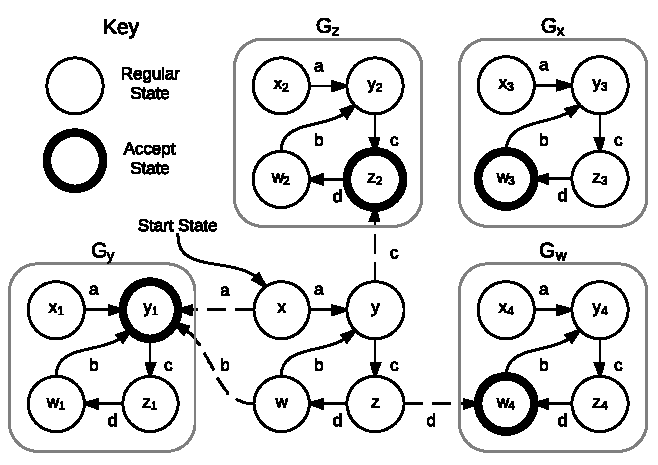
\includegraphics[width=0.6\linewidth]{Ghost2.pdf}
\caption{Corresponding NFA.}
\label{fig:reduction}
\end{figure}

For the other direction of the equivalence, a winning strategy in Ghost (played on the language of the NFA that corresponds to an instance of Generalized Geography) gives a winning strategy in Generalized Geography. The winning strategy in Ghost played on the NFA is to follow valid edges and to avoid ever getting to the accept state of some $G_x$, which corresponds to going back to the same vertex in Generalized Geography.

Thus, the proof follows. 
\end{proof}

\section{Variants}
\label{Variants}

\begin{corollary}
Determining whether player 1 has a winning strategy is in PSPACE in Superghost, Superduperghost, and Xghost mentioned variants of the game.
\end{corollary}

\begin{proof}
We note that we can still reduce the problem to the satisfiability of a fully-quantified boolean formula. We use the same formula, except that now for every player's turn, there are additional variables specifying which position the letter was played at, and/or whether the word fragment was reversed. Since the number of turns is polynomial, there is a polynomial multiplicative overhead in the size of the formula, which is still polynomial. 
\end{proof}

\begin{corollary}
Determining whether player 1 has a winning strategy when Superghost is played over regular languages is PSPACE-hard. 
\end{corollary}

\begin{proof}
We reduce from determining whether player 1 has a winning strategy when Ghost is played over regular language. Given a regular expression, make a new regular expression with the new symbol \# appended twice at the front. This way, no words will have \# in the middle, and so a player cannot place a letter at the begining of the word. Since we've added two symbols at the begining, we maintain the same parity.
\end{proof} 

\begin{corollary}
Determining whether player 1 has a winning strategy when Superduperghost is played over regular languages is PSPACE-hard.
\end{corollary}

\begin{proof}
This reduction is exactly the same as Superghost since if we ever reverse a string, then the \# will be at the end, which is not a valid prefix. 
\end{proof}

\begin{corollary}
Determining whether player 1 has a winning strategy when Xghost is played over regular languages is PSPACE-hard. 
\end{corollary}

\begin{proof}
We can use a similar reduction to the case with Superghost. Given a regular expression of an instance of Ghost, we give a new regular expression that won't allow players to place letters in the middle. We introduce three new symbols into the language @, \% and \&. We place @ at the beginning and between every symbol in the regular expression, we append \% before and \& after the symbol. The @ guarantees that we never append anything at the begining of the word and \% and \& guarantee that there is never any letters appended in the middle. Also, at each point, we always maintain parity.

For example, suppose the regular expression was $a(b^* \cup cd)$, then the transformed expression is
\[ @(\%a\&)((\%b\&)^* \cup (\%c\&)(\%d\&)) \]
\end{proof}

\begin{theorem}
Determining whether player 1 has a winning strategy when Spook is played over regular languages is PSPACE-hard.
\end{theorem}

\begin{proof}
This reduction is a bit different from the previous, since the order does not really matter. In fact, a short modification to this proof will also show PSPACE-hardness for the previous results; however, the previous proofs generalize to the German language nicer. 

The reduction is from Generalized Geography. We will build a regular expression whose language is the words that represent an incorrect history for Generalized Geography. So given a graph $G = (V, E)$ where $|V| = n$, we will have a literal $v_i$ for $v \in V$ and $i \in [n]$. The literal $v_i$ will represent whether the token in Generalized Geography was played on $v$ at turn $i$. The regular expression will contain three parts:

1. We need to check that nodes are only accesses once.
\[ R_1 = \bigcup_{v\in V} \bigcup_{i,j\in [n]}(v_iv_j \Sigma^*) \]

2. We need to check that only nodes with edges to them are accessed.
\[ R_2 = \bigcup_{v, w \in V, (v,w) \notin E} \bigcup_{i \in [n-1]} (v_iw_{i+1}\Sigma^*) \]

3. We need to check that the letters are placed in order.
\[ R_3 = \bigcup_{v, w \in V} \bigcup_{i \in [n] - \{1\}} \left(v_i(\Sigma - \cup_{x \in V} x_{i-1})^* \right) \]

So the expression 
\[ R_1 \cup R_2 \cup R_3 \]
makes the language of all invalid histories of Generalized Geography.

This will ensure that the literals chosen by Spook can be arranged in a line that represents the game play of Generalized Geography. If player 1 wins the game of Spook, then its because player 2 was stuck and couldn't make a valid move. Note that the expression is polynomial length and can be written down in polynomial time. Therefore, the game is PSPACE-hard. 
\end{proof}

\begin{corollary}
Superghost, Superduperghost, and Xghost are all PSPACE-hard when played on subsets of the German language.
\end{corollary}

\begin{proof}
Superghost and Superduperghost have the same reductions when played in German. Since the new symbol \# just becomes another German word of odd length with a different letter. Additionaly, since there is only one German word starting with a unique letter, if a letter is added to the middle, then the word is no longer a valid prefix. 
\end{proof}

\section{Playing on Subsets of German}

\subsection{Concatenating Words}



It turns out that the idea behind the proof of Theorem 1 can be used to show that Ghost is PSPACE-hard when played on subsets of the German language. We choose to focus on the German language because in German, multiple nouns can always be concatenated together to make new nouns. For example, ``wort", ``band", and ``teil" are all valid German nouns, and thus concatenations such as “wortband” and “wortteilband” are also valid nouns \cite{german}. Therefore, we can describe subsets of the German language with regular expressions.

We consider the following instance of Ghost: The game is played over a given subset of the German language. Does player 1 have a winning strategy if he/she is first to pick a letter?

\begin{theorem}Determining whether player 1 has a winning strategy when Ghost is played over subsets of the German language is PSPACE-hard.
\end{theorem}

\begin{proof} The reduction is very similar in structure to the reduction used in the proof of Theorem 1. However, here we consider Planar Generalized Geography, which is still PSPACE-hard \cite{Sipser}. Given an instance of Planar Generalized Geography, we can four-color the graph in polynomial time \cite{planargraph}. Each edge is then labeled with the color of the vertex it points to. Given this labeling of the graph, we build a corresponding NFA following the procedure in the proof of Theorem 1. The only change we make is that the labels in the graph are mapped to German nouns of odd length that start with different letters. We choose the nouns ``krankenhaus" (hospital), ``wiedervereinigung" (reunification), ``tod" (death), and ``m{\"a}dchen" (girl). Thus, all edges that are colored one color will give transitions labeled with ``tod"��, for example. 

	The German language allows nouns to be concatenated, so the subset of words that are accepted in the NFA are grammatically valid German words. Since the words are all of odd length, when the word finishes, the next player can pick the next word. This corresponds to picking an edge in the NFA, except each transition may take multiple turns. Also, since the starting letter of the words are different, once you start a word, the whole word is specified. This construction builds an NFA that accepts a subset of the words in the German language. 
\end{proof}

\section{Conclusion}
\label{Conclusion}

We determined that playing Ghost over regular languages is PSPACE-hard, and we used the same reduction structure to show that Ghost played over subsets of the German language is also PSPACE-hard. The first result is somewhat abstract, as Ghost is generally not played over arbitrary regular languages. However, the second result indicates that there may be other real-world languages that Ghost is hard to play over.

There is one more variant of Ghost that we did not analyze which would be interesting to think about. Spook is similar to Ghost, except that instead of keeping a prefix of a word, we just keep a bag of letters and we want to avoid having the letters in the bag make a word, regardless of the order.

\subsubsection*{Acknowledgments.} This paper began as a final project for the MIT class ``The Mathematics of Toys and Games", taught by Jayson Lynch and Robert Sloan and supervised by Erik D. Demaine. We thank them for helpful dicussions on this topic.

\bibliography{references}
\bibliographystyle{plain}

\end{document}
